\documentclass[convert={density=300,outext=.png}]{standalone}
\usepackage{tikz}

\begin{document}
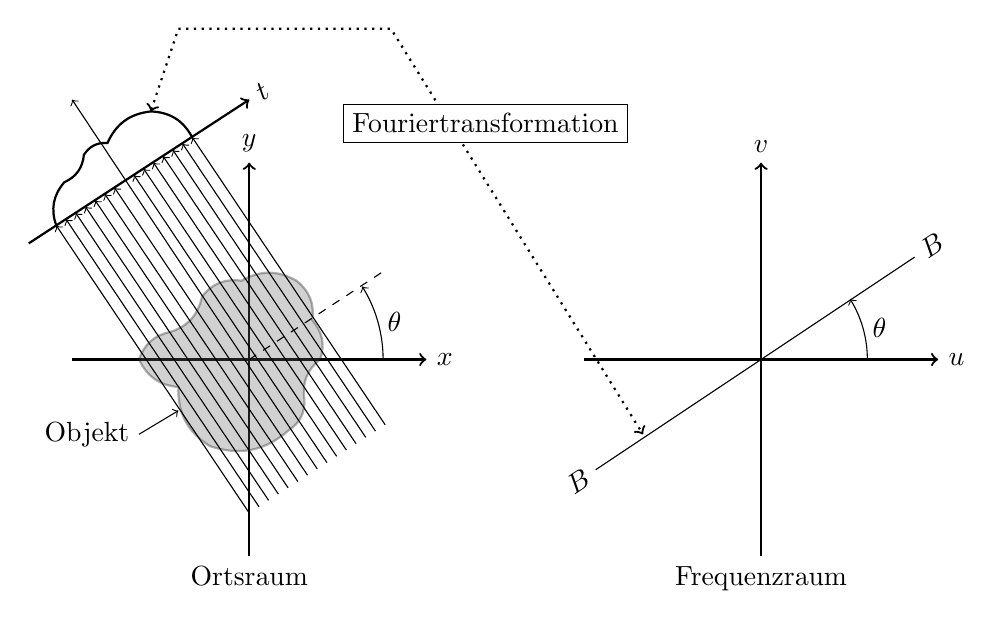
\begin{tikzpicture}[axis/.style={thick,->}]
    % links
    \draw[axis] (-5.5, 0) -- (-1, 0) node [right] {$x$};
    \draw[axis] (-3.25, -2.5) -- (-3.25, 2.5) node[pos=0,below] {Ortsraum} node [above] {$y$};

    % Objekt
    \draw[thick,fill=black!60!white,opacity=0.3] (-2.35, 0) to [bend right] (-2.45, 0.5) to [bend right] (-2.65, 1)
                                                            to [bend right] (-3.35, 1) to [bend right] (-3.85, 0.8)
                                                            to [bend left] (-4.25, 0.35) to [bend right] (-4.65, 0)
                                                            to [bend right] (-4.15 ,-0.35)
                                                            to [bend right] (-3.75, -1.1)
                                                            to [bend right] (-2.75, -0.9)
                                                            to [bend right] (-2.55 ,-0.5)
                                                            to [bend left] (-2.35, 0);
    \draw[->] (-4.65, -0.95) -- (-4.15, -0.65) node[pos=0, left] {Objekt};

    % Detektor
    \draw[axis] (-6.05, 1.475) -- (-3.25, 3.3) node[pos=1,sloped,right] {$t$};
    \draw[thick] (-5.7, 1.7) to [bend left] (-5.6, 2.25) to [bend right] (-5.35, 2.6)
    to [bend left] (-5.05, 2.75) to [bend left] (-4.5, 3.15)
    to [bend left] (-3.9733333333333, 2.82);

    % Pfeile zum Detektor
    \foreach \w in {0,...,6}
        \draw[->] (-3.25 + \w * 0.1233333333333, -1.95 + \w * 0.08)
                  -- (-5.7 + \w * 0.1233333333333, 1.7 + \w * 0.08);
    \draw[->] (-3.25 + 7 * 0.1233333333333, -1.95 + 7 * 0.08) -- (-5.5, 3.3);
    \foreach \w in {8,...,14}
        \draw[->] (-3.25 + \w * 0.1233333333333, -1.95 + \w * 0.08)
                  -- (-5.7 + \w * 0.1233333333333, 1.7 + \w * 0.08);

    % Linie
    \draw[dashed] (-3.25, 0) -- (-1.5, 1.15);

    % Winkel
    \draw[->] (-1.55, 0) arc(0:32:17.5mm) node[pos=0.5,right] {$\theta$};

    % rechts
    \draw[axis] (1, 0) -- (5.5, 0) node [right] {$u$};
    \draw[axis] (3.25, -2.5) -- (3.25, 2.5) node [pos=0,below] {Frequenzraum} node [above] {$v$};

    % Linie
    \draw (1.15, -1.4) -- (5.2, 1.3) node[sloped,pos=0,left] {$B$} node[sloped,pos=1,right] {$B$};

    % Winkel
    \draw[->] (4.6, 0) arc (0:32:14.5mm) node[pos=0.5,right] {$\theta$};

    % Verbindung
    \draw[<->,dotted,thick] (-4.5, 3.15) -- (-4.15, 4.2) -- (-1.45, 4.2) -- (1.75, -0.95);
    \node[draw,fill=white] at (-0.25, 3) {Fouriertransformation};
\end{tikzpicture}
\end{document}
